\section{Chi-Square Probability Table}
\label{chiSquareProbabilityTable}

A \term{chi-square probability table} may be used
to find tail areas of a chi-square distribution.
The \term{chi-square table} is partially shown in
Figure~\ref{chiSquareProbabilityTableShort},
and the complete table may be found on
page~\pageref{fullChiSqTable}.
When using a chi-square table, we examine a particular
row for distributions
with different degrees of freedom, and we identify a range for
the area (e.g. 0.025 to 0.05).
Note that the chi-square table provides upper tail values,
which is different than the normal and $t$-distribution tables.

\begin{figure}[h]
\centering
\begin{tabular}{r | rrrr | rrrr |}
  \hline
Upper tail & 0.3 & 0.2 & 0.1 & 0.05 & 0.02 & 0.01 & 0.005 & 0.001 \\ 
  \hline
%df \hfill 1 & \footnotesize 1.07 & \footnotesize 1.64 & \footnotesize 2.71 & \footnotesize 3.84 & \footnotesize 5.41 & \footnotesize 6.63 & \footnotesize 7.88 & \footnotesize 10.83 \\ 
df \hfill 2 & \footnotesize 2.41 & \footnotesize \highlightO{3.22} & \footnotesize \highlightO{4.61} & \footnotesize 5.99 & \footnotesize 7.82 & \footnotesize 9.21 & \footnotesize 10.60 & \footnotesize 13.82 \\ 
  \em3 & \em\footnotesize 3.66 & \em\footnotesize 4.64 & \em\footnotesize \highlightT{6.25} & \em\footnotesize 7.81 & \em\footnotesize 9.84 & \em\footnotesize 11.34 & \em\footnotesize 12.84 & \em\footnotesize 16.27 \\ 
  4 & \footnotesize 4.88 & \footnotesize 5.99 & \footnotesize 7.78 & \footnotesize 9.49 & \footnotesize 11.67 & \footnotesize 13.28 & \footnotesize 14.86 & \footnotesize 18.47 \\ 
  5 & \footnotesize 6.06 & \footnotesize 7.29 & \footnotesize 9.24 & \footnotesize 11.07 & \footnotesize 13.39 & \footnotesize 15.09 & \footnotesize 16.75 & \footnotesize 20.52 \\ 
  \hline
  6 & \footnotesize 7.23 & \footnotesize 8.56 & \footnotesize 10.64 & \footnotesize 12.59 & \footnotesize 15.03 & \footnotesize 16.81 & \footnotesize 18.55 & \footnotesize 22.46 \\ 
  7 & \footnotesize 8.38 & \footnotesize 9.80 & \footnotesize 12.02 & \footnotesize 14.07 & \footnotesize 16.62 & \footnotesize 18.48 & \footnotesize 20.28 & \footnotesize 24.32 \\ 
  \hline
\end{tabular}
\caption{A section of the chi-square table. A complete table is in Appendix~\ref{chiSquareProbabilityTable}.}
\label{chiSquareProbabilityTableShort}
\end{figure}

\begin{examplewrap}
\begin{nexample}{Figure~\ref{app_chiSquareAreaAbove6Point25WithDF3}
    shows a chi-square distribution with 3 degrees of freedom
    and an upper shaded tail starting at 6.25.
    Use Figure~\ref{chiSquareProbabilityTableShort}
    to estimate the shaded area.}
  This distribution has three degrees of freedom,
  so only the row with 3 degrees of freedom (df) is relevant.
  This row has been italicized in the table.
  Next, we see that the value -- 6.25 -- falls in the column
  with upper tail area 0.1.
  That is, the shaded upper tail of
  Figure~\ref{app_chiSquareAreaAbove6Point25WithDF3}
  has area 0.1.

  This example was unusual, in that we observed the
  \emph{exact} value in the table.
  In the next examples, we encounter situations where
  we cannot precisely estimate the tail area and must
  instead provide a range of values.
\end{nexample}
\end{examplewrap}

\begin{figure}
\centering
\subfigure[]{
\includegraphics[width=0.475\textwidth]{ch_inference_for_props/figures/arrayOfFigureAreasForChiSquareDistribution/chiSquareAreaAbove6Point25WithDF3/chiSquareAreaAbove6Point25WithDF3}
\label{app_chiSquareAreaAbove6Point25WithDF3}
}
\subfigure[]{
\includegraphics[width=0.475\textwidth]{ch_inference_for_props/figures/arrayOfFigureAreasForChiSquareDistribution/chiSquareAreaAbove4Point3WithDF2/chiSquareAreaAbove4Point3WithDF2}
\label{app_chiSquareAreaAbove4Point3WithDF2}
}
\subfigure[]{
\includegraphics[width=0.475\textwidth]{ch_inference_for_props/figures/arrayOfFigureAreasForChiSquareDistribution/chiSquareAreaAbove5Point1WithDF5/chiSquareAreaAbove5Point1WithDF5}
\label{app_chiSquareAreaAbove5Point1WithDF5}
}
\subfigure[]{
\includegraphics[width=0.475\textwidth]{ch_inference_for_props/figures/arrayOfFigureAreasForChiSquareDistribution/chiSquareAreaAbove11Point7WithDF7/chiSquareAreaAbove11Point7WithDF7}
\label{app_chiSquareAreaAbove11Point7WithDF7}
}
%\subfigure[]{
%\includegraphics[width=0.475\textwidth]{ch_inference_for_props/figures/arrayOfFigureAreasForChiSquareDistribution/chiSquareAreaAbove10WithDF4/chiSquareAreaAbove10WithDF4}
%\label{app_chiSquareAreaAbove10WithDF4}
%}
%\subfigure[]{
%\includegraphics[width=0.475\textwidth]{ch_inference_for_props/figures/arrayOfFigureAreasForChiSquareDistribution/chiSquareAreaAbove9Point21WithDF3/chiSquareAreaAbove9Point21WithDF3}
%\label{app_chiSquareAreaAbove9Point21WithDF3}
%}
\caption{
\textbf{\subref{app_chiSquareAreaAbove6Point25WithDF3}}~Chi-square distribution with 3~degrees of freedom, area above 6.25 shaded.
\textbf{\subref{app_chiSquareAreaAbove4Point3WithDF2}}~2~degrees of freedom, area above 4.3 shaded.
\textbf{\subref{app_chiSquareAreaAbove5Point1WithDF5}}~5~degrees of freedom, area above 5.1 shaded.
\textbf{\subref{app_chiSquareAreaAbove11Point7WithDF7}}~7~degrees of freedom, area above 11.7 shaded.
%\textbf{\subref{app_chiSquareAreaAbove10WithDF4}}~4~degrees of freedom, area above 10 shaded.
%\textbf{\subref{app_chiSquareAreaAbove9Point21WithDF3}}~3~degrees of freedom, area above 9.21 shaded.
}
\label{arrayOfFigureAreasForChiSquareDistributionChiSqAppendix}
\end{figure}

\begin{examplewrap}
\begin{nexample}{
    Figure~\ref{app_chiSquareAreaAbove4Point3WithDF2}
    shows the upper tail of a chi-square distribution
    with 2~degrees of freedom.
    The area above value 4.3 has been shaded;
    find this tail area.}
  The cutoff 4.3 falls between the second and third columns
  in the 2~degrees of freedom row.
  Because these columns correspond to tail areas of 0.2 and 0.1,
  we can be certain that the area shaded in
  Figure~\ref{app_chiSquareAreaAbove4Point3WithDF2}
  is between 0.1 and 0.2.
\end{nexample}
\end{examplewrap}

\begin{examplewrap}
\begin{nexample}{Figure~\ref{app_chiSquareAreaAbove5Point1WithDF5} shows an upper tail for a chi-square distribution with 5 degrees of freedom and a cutoff of 5.1. Find the tail area.}
Looking in the row with 5 df, 5.1 falls below the smallest cutoff for this row (6.06). That means we can only say that the area is \emph{greater than} 0.3.
\end{nexample}
\end{examplewrap}

\begin{examplewrap}
\begin{nexample}{Figure~\ref{app_chiSquareAreaAbove11Point7WithDF7}
    shows a cutoff of 11.7 on a chi-square distribution with
    7~degrees of freedom.
    Find the area of the upper tail.}
  The value 11.7 falls between 9.80 and 12.02 in the 7 df row.
  Thus, the area is between 0.1 and 0.2.
\end{nexample}
\end{examplewrap}

%\begin{exercisewrap}
%\begin{nexercise}
%Figure~\ref{app_chiSquareAreaAbove10WithDF4} shows a cutoff of 10 on a chi-square distribution with 4 degrees of freedom. Find the area of the upper tail.\footnotemark
%\end{nexercise}
%\end{exercisewrap}
%\footnotetext{The area is between 0.02 and 0.05.}
%
%\begin{exercisewrap}
%\begin{nexercise}
%Figure~\ref{app_chiSquareAreaAbove9Point21WithDF3} shows a cutoff of 9.21 with a chi-square distribution with 3 df. Find the area of the upper tail.\footnotemark
%\end{nexercise}
%\end{exercisewrap}
%\footnotetext{Between 0.02 and 0.05.}

%\begin{figure}[hhh]
%\centering
%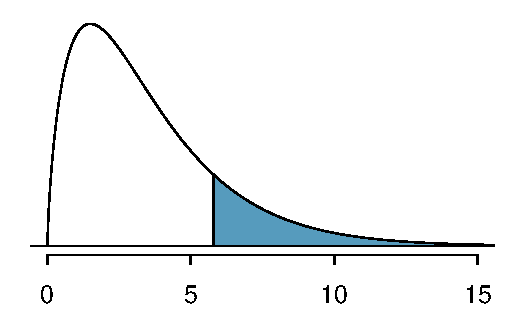
\includegraphics[height=1.5in]{extraTeX/tables/figures/chiSquareTail/chiSquareTail}
%\caption{Areas in the chi-square table always refer to the right tail.}
%\end{figure}

\begin{center}
\begin{tabular}{r | rrrr | rrrr |}
  \hline
Upper tail & 0.3 & 0.2 & 0.1 & 0.05 & 0.02 & 0.01 & 0.005 & 0.001 \\ 
  \hline
df \hfill 1 & \footnotesize 1.07 & \footnotesize 1.64 & \footnotesize 2.71 & \footnotesize 3.84 & \footnotesize 5.41 & \footnotesize 6.63 & \footnotesize 7.88 & \footnotesize 10.83 \\ 
  2 & \footnotesize 2.41 & \footnotesize 3.22 & \footnotesize 4.61 & \footnotesize 5.99 & \footnotesize 7.82 & \footnotesize 9.21 & \footnotesize 10.60 & \footnotesize 13.82 \\ 
  3 & \footnotesize 3.66 & \footnotesize 4.64 & \footnotesize 6.25 & \footnotesize 7.81 & \footnotesize 9.84 & \footnotesize 11.34 & \footnotesize 12.84 & \footnotesize 16.27 \\ 
  4 & \footnotesize 4.88 & \footnotesize 5.99 & \footnotesize 7.78 & \footnotesize 9.49 & \footnotesize 11.67 & \footnotesize 13.28 & \footnotesize 14.86 & \footnotesize 18.47 \\ 
  5 & \footnotesize 6.06 & \footnotesize 7.29 & \footnotesize 9.24 & \footnotesize 11.07 & \footnotesize 13.39 & \footnotesize 15.09 & \footnotesize 16.75 & \footnotesize 20.52 \\ 
  \hline
  6 & \footnotesize 7.23 & \footnotesize 8.56 & \footnotesize 10.64 & \footnotesize 12.59 & \footnotesize 15.03 & \footnotesize 16.81 & \footnotesize 18.55 & \footnotesize 22.46 \\ 
  7 & \footnotesize 8.38 & \footnotesize 9.80 & \footnotesize 12.02 & \footnotesize 14.07 & \footnotesize 16.62 & \footnotesize 18.48 & \footnotesize 20.28 & \footnotesize 24.32 \\ 
  8 & \footnotesize 9.52 & \footnotesize 11.03 & \footnotesize 13.36 & \footnotesize 15.51 & \footnotesize 18.17 & \footnotesize 20.09 & \footnotesize 21.95 & \footnotesize 26.12 \\ 
  9 & \footnotesize 10.66 & \footnotesize 12.24 & \footnotesize 14.68 & \footnotesize 16.92 & \footnotesize 19.68 & \footnotesize 21.67 & \footnotesize 23.59 & \footnotesize 27.88 \\ 
  10 & \footnotesize 11.78 & \footnotesize 13.44 & \footnotesize 15.99 & \footnotesize 18.31 & \footnotesize 21.16 & \footnotesize 23.21 & \footnotesize 25.19 & \footnotesize 29.59 \\ 
  \hline
  11 & \footnotesize \footnotesize 12.90 & \footnotesize 14.63 & \footnotesize 17.28 & \footnotesize 19.68 & \footnotesize 22.62 & \footnotesize 24.72 & \footnotesize 26.76 & \footnotesize 31.26 \\ 
  12 & \footnotesize 14.01 & \footnotesize 15.81 & \footnotesize 18.55 & \footnotesize 21.03 & \footnotesize 24.05 & \footnotesize 26.22 & \footnotesize 28.30 & \footnotesize 32.91 \\ 
  13 & \footnotesize 15.12 & \footnotesize 16.98 & \footnotesize 19.81 & \footnotesize 22.36 & \footnotesize 25.47 & \footnotesize 27.69 & \footnotesize 29.82 & \footnotesize 34.53 \\ 
  14 & \footnotesize 16.22 & \footnotesize 18.15 & \footnotesize 21.06 & \footnotesize 23.68 & \footnotesize 26.87 & \footnotesize 29.14 & \footnotesize 31.32 & \footnotesize 36.12 \\ 
  15 & \footnotesize 17.32 & \footnotesize 19.31 & \footnotesize 22.31 & \footnotesize 25.00 & \footnotesize 28.26 & \footnotesize 30.58 & \footnotesize 32.80 & \footnotesize 37.70 \\ 
  \hline
  16 & \footnotesize 18.42 & \footnotesize 20.47 & \footnotesize 23.54 & \footnotesize 26.30 & \footnotesize 29.63 & \footnotesize 32.00 & \footnotesize 34.27 & \footnotesize 39.25 \\ 
  17 & \footnotesize 19.51 & \footnotesize 21.61 & \footnotesize 24.77 & \footnotesize 27.59 & \footnotesize 31.00 & \footnotesize 33.41 & \footnotesize 35.72 & \footnotesize 40.79 \\ 
  18 & \footnotesize 20.60 & \footnotesize 22.76 & \footnotesize 25.99 & \footnotesize 28.87 & \footnotesize 32.35 & \footnotesize 34.81 & \footnotesize 37.16 & \footnotesize 42.31 \\ 
  19 & \footnotesize 21.69 & \footnotesize 23.90 & \footnotesize 27.20 & \footnotesize 30.14 & \footnotesize 33.69 & \footnotesize 36.19 & \footnotesize 38.58 & \footnotesize 43.82 \\ 
  20 & \footnotesize 22.77 & \footnotesize 25.04 & \footnotesize 28.41 & \footnotesize 31.41 & \footnotesize 35.02 & \footnotesize 37.57 & \footnotesize 40.00 & \footnotesize 45.31 \\ 
  \hline
  25 & \footnotesize 28.17 & \footnotesize 30.68 & \footnotesize 34.38 & \footnotesize 37.65 & \footnotesize 41.57 & \footnotesize 44.31 & \footnotesize 46.93 & \footnotesize 52.62 \\ 
  30 & \footnotesize 33.53 & \footnotesize 36.25 & \footnotesize 40.26 & \footnotesize 43.77 & \footnotesize 47.96 & \footnotesize 50.89 & \footnotesize 53.67 & \footnotesize 59.70 \\ 
  40 & \footnotesize 44.16 & \footnotesize 47.27 & \footnotesize 51.81 & \footnotesize 55.76 & \footnotesize 60.44 & \footnotesize 63.69 & \footnotesize 66.77 & \footnotesize 73.40 \\ 
  50 & \footnotesize 54.72 & \footnotesize 58.16 & \footnotesize 63.17 & \footnotesize 67.50 & \footnotesize 72.61 & \footnotesize 76.15 & \footnotesize 79.49 & \footnotesize 86.66 \\ 
  \hline
\end{tabular}
\label{fullChiSqTable}
\end{center}
